\documentclass{article}

% packages and configurations
\usepackage{hyperref}
\usepackage{animate} % needed for animations and videos
\usepackage{bm} % bold font in equation environments
\usepackage[utf8]{inputenc}	% für Umlaute ect.
\usepackage{fancyhdr} % für header
\usepackage{lastpage} % für footer
\usepackage{extramarks} % für header und footer
\usepackage{amsthm} % math stuff
\usepackage{amsmath} % math stuff
\usepackage{amssymb} % math stuff
\usepackage{color}
\usepackage[procnames]{listings} % code listings
\usepackage{graphicx} % für graphics
\usepackage[toc]{glossaries} % Glossar
\usepackage{color}
\usepackage{tikz}
\usepackage[absolute,overlay]{textpos} %to translate graphics through space
\usepackage{soul}
\usepackage{xcolor}
\usepackage{textpos}
\usepackage{caption}
\usepackage{parcolumns}
\usepackage{enumerate}
\usepackage[ngerman]{babel} % Umlaute
\usepackage[T1]{fontenc}    % this is needed for correct output of umlauts in pd
\usepackage[section]{placeins} %forces placeins to stay in section
\usepackage{datetime} % custom dates
\usepackage{afterpage}
\usepackage[section]{placeins}

\definecolor{keywords}{RGB}{255,0,90}
\definecolor{comments}{RGB}{0,0,113}
\definecolor{red}{RGB}{160,0,0}
\definecolor{green}{RGB}{0,150,0}

\lstset{language=Python, 
	basicstyle=\ttfamily\small, 
	keywordstyle=\color{keywords},
	commentstyle=\color{comments},
	stringstyle=\color{red},
	showstringspaces=false,
	identifierstyle=\color{green},
	procnamekeys={def,class}}

\title{Bringing together visual analytics and probabilistic programming languages}
\author{Jonas Aaron Gütter  \\
	Friedrich Schiller Universität Jena  \\
    Matrikelnr 152127 \\
    Prof.Dr. Joachim Giesen \\
    M. Sc. Phillip Lucas
	}

\makeglossaries


\begin{document}


\maketitle

\begin{abstract}
A probabilistic programming language (PPL) provides methods to represent a probabilistic model by using the full power of a general purpose programming language. Thereby it is possible to specify complex models with a comparatively low amount of code. With Uber, Microsoft and DARPA focusing research efforts towards this area, PPLs are likely to play an important role in science and industry in the near future.
However in most cases, models built by PPLs lack appropriate ways to be properly visualized, although visualization is an important first step in detecting errors and assessing the overall fitness of a model. This could be resolved by the software Lumen, developed by Philipp Lucas, which provides several visualization methods for statistical models. PPLs are not yet supported by Lumen, and the goal of the master thesis at hand is to change that by implementing an interface between Lumen and a chosen PPL, so that exploring PPL models by visual analytics becomes possible.
The thesis will be divided into two main parts, the first part being an overview about how PPLs work and what existing PPLs there are available. Out of these, the most appropriate one will be chosen for the task. The second, more practical part will then document the actual implementation of the interface.

\end{abstract}

\tableofcontents

\newglossaryentry{Bayesian network}
{
  name=Bayesian network,
  description={...}
}

\newglossaryentry{conditional probability distribution}
{
  name=conditional probability distribution,
  description={...}
}

\newglossaryentry{inference algorithm}
{
  name=inference algorithm,
  description={is a key part of a \gls{probabilistic reasoning system}}
}

\newglossaryentry{joint probability distribution}
{
  name=joint probability distribution,
  description={...}
}

\newglossaryentry{marginal distribution}
{
  name=marginal distribution,
  description={...}
}

\newglossaryentry{probabilistic model}
{
  name=probabilistic model,
  description={is a key part of a \gls{probabilistic reasoning system}}
}

\newglossaryentry{probabilistic programming}
{
  name=probabilistic programming,
  description={is something}
}

\newglossaryentry{probabilistic programming language}
{
  name=probabilistic programming language,
  description={is used to create a \gls{probabilistic reasoning system} more effectively than with a conventional programming language}
}

\newglossaryentry{probabilistic reasoning system}
{
  name=probabilistic reasoning system,
  description={consists of a \gls{probabilistic model} and an \gls{inference algorithm}}
}

\newglossaryentry{Turing-complete}
{
  name=Turing-complete,
  description={a turing-complete machine can perform any computation that could theoretically performed by any computer. universally programmable.}
}
\printglossaries
\section{Road Map}

\begin{enumerate}
	\item Getting started
	\begin{itemize}
		\item set up Master thesis document
		\item Probabilistic Programming Languages
		\begin{itemize}
			\item play at least with: PyMC3, Stan
			\item read the docs, wiki, ...
			\item download the libraries
			\item reproduce the getting started tutorials
			\item --> understand the ideas and how to use it, get a feeling for it
		\end{itemize}
		\item theoretic background: Read Bayesian Data Analysis part I, Chapter 1,2 and part II, chapter 6,7
		\item Lumen
		\begin{itemize}
			\item install locally and play with
			\item understand main idea of Lumen and what we want to do with it
		\end{itemize}
		\item Start filling up your MA thesis document
		\begin{itemize}
			\item understand and write down in MA thesis the "why \& what"
			\item describe the background of the work, e.g. summarize PPLs
		\end{itemize}
		\item give a short presentation
		\begin{itemize}
			\item what have you done and learned
			\item what do you plan to do?
			\item why is it relevant?
			\item how do you plan to measure the success?
		\end{itemize}	
	\end{itemize}
	\item First connection of PPLs to Lumen
	\begin{itemize}
		\item Start from small, very simple and specific example. Generalize later.
		\item Choose PPL to work with
		\begin {itemize}
		\item work out requirements on PPL
		\item work out preferred features of PPL
		\item choose a PPL based on these requrements and preferences
	\end{itemize}
	\item design wrapper of PPL with Lumen
	\begin{itemize}
		\item work out requirement and interface
		\item identify necessary work on Lumen
		\item identify necessary work
	\end{itemize}
	\item Connect chosen specific example with lumen
	\item Continue to work on your master thesis document!
\end{itemize}
\item Improve, generalize and clean up the connection of your PPL to Lumen
\end{enumerate}

\section{Introduction}

\textit{In this section, the motivation for the thesis is explained, the task of the thesis is made clear. Furthermore, the structure of the thesis is outlined here. It is possible to get the basic ideas and results of the thesis from reading only this section and the conclusion.}
\\
\\
In Bayesian data analysis we have a prior distribution for the parameters, $p(\theta)$, which represents our knowledge about them without seeing any data. We have also the likelihood of our data, $p(X|\theta)$, which represents the probability of obtaining the data $X$ given the parameter $\theta$. Using the Bayes' rule, we can then compute the posterior distribution for $\theta$, $p(X|\theta)$:

\begin{equation}
p(\theta|X) = p(X|\theta) * p(\theta) / p(X)
\end{equation}

Since the posterior distribution for $\theta$ can often not be computed analytically, Probabilistic Programming Languages use sampling methods to approximate the posterior distribution for $\theta$.

When we want to visualize parameters and data, and also want to condition and marginalize arbitrarily, we need the joint distribution $p(x,\theta|X)$. The joint distribution can be computed by:

\begin{equation}
p(x,\theta|X) = p(x|\theta) * p(\theta|X)
\end{equation}

The posterior distribution of the parameters, $p(\theta|X)$, can be approximated by PPLs through sampling, as stated above. (--> Make sure that this is true!!). To get density values from samples, we have to perform density estimation methods \url{http://scikit-learn.org/stable/modules/generated/sklearn.neighbors.KernelDensity.html#sklearn.neighbors.KernelDensity.score_samples}

\section{Concepts of Bayesian Statistics}

\textit{Theoretical concepts of building statistical models using a Bayesian approach are explained in this section. Also graphical model checking is treated here, as that will be the common use case for the Lumen interface created in this thesis.}
\\
\\
%In the field of statistics, one deals usually with the following questions:
%
%\begin{itemize}
%	\item What kind of model should I choose?
%	\item Which features should I include in my model?
%	\item What are the most likely values for my model parameters?
%	\item What is the most likely outcome for additional observations under certain conditions?
%	\item How certain am I that my estimated parameter values are correct?
%\end{itemize}
%The latter three of these questions can be answered by using a Bayesian approach to statistics. Given a model, Bayesian statistics is about computing a joint probability distribution over all parameters and outcomes, so that a probability density for each possible value of parameters and outcomes can be obtained. Prior knowledge of the problem as well as observed data affect the form of the joint probability distribution. Using marginalization, conditional probability distributions can then be calculated for the desired outcomes. These conditional probability distributions are also called posteriors and can be used for parameter estimation, prediction and assessing the uncertainty of estimates. This chapter will outline how Bayesian statistics are applied to answer the abovementioned questions.
\subsection{Rules of Probabilistic Inference}

When working with Bayesian models, it will be necessary to transform conditional, marginal and joint distributions into one another. There are three rules of probabilistic inference which achieve this: The chain rule, the total probability rule, and the Bayes' rule. The following explanations are taken from \cite{9781617292330}.

\subsubsection{Chain rule}

The chain rule is used to calculate a \gls{joint probability distribution} of several variables from local \gls{conditional probability distribution}s of these variables:

\begin{equation}
P(X_1 ,X_2 ,...X_n ) = P(X_1 )P(X_2 | X_1 )P(X_3 | X_1 ,X_2 )...P(X_n | X_1 ,X_2 ,...X_{n-1}) )
\end{equation}

\subsubsection{Total probability rule}

The total probability rule calculates the probability distribution over a subset of variables, also called a \gls{marginal distribution}, by summing out all the other variables, that is by summing the probability distributions for each combination of values of these variables:

\begin{equation}
P(\boldsymbol X |\boldsymbol Z ) = \sum_{\boldsymbol y}   P(\boldsymbol X ,\boldsymbol Y =\boldsymbol y |\boldsymbol Z )
\end{equation} 

\subsubsection{Bayes' rule}

Bayes' rule calculates the probability of a cause, given an effect, by using the prior probability of the cause and the probability of the effect, given the cause. 

\begin{equation}
P(X|Y) = ( P(Y|X) * P(X) ) / P(Y)
\end{equation}

\subsection{General principle}
Goal of Bayesian Statistics: Setting up a probability model over model parameters and observed data

When doing Bayesian data analysis, we have observed data $Y$ and a prior belief $P(\theta)$ about the mechanism that generated the data, and we use those to set up a full probability model $P(y,\theta|Y)$ over all model parameters $\theta$ and all possible data $y$. The conceptual difference to conventional Statistics is two-fold: First, we don't use prior beliefs in conventional Statistics (at least not for parameter estimation), second, in conventional Statistics we only set up a probability model over the data, not over the model parameters. The model parameters in conventional Statistics are fixed after the parameter estimation.
\\
\\
The principle of setting up the full probability model of Bayesian Statistics (also called the joint probability distribution) is as follows:
\\
According to the chain rule, we can compute the full probability model with the following formula:
\begin{equation}
p(y,\theta|Y) = p(y|\theta,Y) * p(\theta|Y)
\end{equation}
Since the probability for a specific value of $y$ does not depend on the observed data $Y$, if we already know $\theta$, we can write equivalently:
\begin{equation}
p(y,\theta|Y) = p(y|\theta) * p(\theta|Y)
\end{equation}
$p(y|\theta)$ is usually easy to compute since it is given by the chosen model class. For computing the second term, $P(\theta|Y)$, we use the Bayes rule:
\begin{equation}
p(\theta|Y) = p(Y|\theta) * p(\theta) / p(Y)
\end{equation}
This is where the prior belief comes into play.

\subsection{Choosing an appropriate prior distribution}
There are two interpretations of prior distributions. The \textit{population} interpretation, where the prior distribution is thought of as a population of possible parameters, from where the current parameter is drawn. This, as far as I understand, requires the range of possible values to be known, e.g from past experience. On the other hand, the \textit{state of knowledge} interpretation looks at the prior distribution as an expression of the user's knowledge or uncertainty, so that the assumption is plausible, that the real parameter value is taken from a random realization of the prior distribution.
\\
When we have lots of knowledge about the parameter already, it makes sense to choose an \textit informative prior, which has a big influence on the posterior distribution.On the other hand, if one does not want prior beliefs to affect the outcome of an analysis, one should not choose informative priors, even when lots of knowledge is available. E.g. when testing a hypothesis, it is not wise to include information in the prior that supports the hypothesis for fairness reasons(?? look that up again on p. 56.). If there is no sufficient data to estimate a prior, it is desirable to choose a prior that is \textit noninformative, meaning that it will contribute very little to the posterior distribution ('let the data speak for itself'). A common noninformative prior, motivated by Laplace's principle of insufficient reason, is the uniform distribution. However, the uniform distribution is not ideal since it is dependent on the parametrization: Applying a uniform distribution to $p(x)$ leads to a non-uniform distribution when looking at $p(x^2)$ and the other way round \cite{1439840954}. Jeffrey's approach to find noninformative prior distributions negates this problem by choosing a prior that is invariant to the parameterization (see https://eventuallyalmosteverywhere.wordpress.com/2013/05/10/bayesian-inference-and-the-jeffreys-prior/).
Besides informative and noninformative prior distributions there is also the \textit {weakly informative} prior distribution. This kind of prior does affect the posterior distribution in terms of regularization (e.g. it prevents extreme outliers), but it does not contain any further special knowledge about the parameter. A normal distribution with high variance is often used as weakly informative prior.
\\
The parameters of the prior distributions are called hyperparameters. The property that prior and posterior distribution are of the parametric form (e.g., both are a beta distribution) (for a given likelihood distribution), is called conjugacy. Conjugate prior distributions have the advantages of being computationally convenient and being intertpretable as additional data.
\\
A prior distribution is called \textit{proper} if it does not depend on data and sums to 1 \cite{1439840954}. Proper distributions can be normalized. The uniform prior for example is \textit{improper}, since it can't be normalized.

\subsection{Sampling distribution}

The sampling distribution, also called the likelihood of the data.
\\
Often it is about which distribution class should be chosen for the prior and the likelihood. Standard, convenient distributions for single-parameter models: normal, binomial, Poisson, exponential. Those can also be combined to represent more complex distributions. For different classes of sampling distributions there are corresponding conjugate prior distributions which lead in turn to posterior distributions of the same form. \cite{1439840954}
\\
distributions can be chosen for mathematical convenience. One could estimate hyperparameters of the likelihood distribution from the data in some cases. This is a bit of a circular reasoning, but apparently  it is appropriate for \cite{1439840954}.

\subsection{Evaluating models}

Since ``all models are wrong", it is necessary, after a Bayesian model has been found, to capture the extent to which the model fails to describe reality. In Bayesian analysis, both the prior and the likelihood distribution can be sources of error.

Different models can lead to different posterior inferences, even if both models have a good fit.

model checking: How good does the model fit the data?
Sensitivitiy analysis: Comparison of different models with good fit

This is necessary after a joint probability density and a posterior density are calculated. How good are the prior and the likelihood model?
\textit{Sensitivity analysis} deals with the question, how much the posterior is changed when one chooses a different (but also reasonable) model for the likelihood or the prior, or other assumptions affecting the posterior.

In theory: Setting up a 'super-model' as joint-distribution which includes all possible realities. Posterior of this super-model then automatically incorporates the sensitivity analysis. In practice this is conceptually and computationally infeasible and also is still dependent on the assumptions made when creating the super-model being correct.

One way is just to compare model predictions with the actual outcomes (this is referred to as external validation). If for some reason it is not possible to get the acutal outcomes (for example if they lie in the future), one needs to approximate external validation with the available data.

\textit{Posterior predictive checking}: Use global summaries of the data distribution and the predictive distribution to evaluate the model: Draw random samples from the predictive distribution, compare e.g. the smallest of these values with the smallest value in the data...

model checking by calculating \textit{test quantities}. \textit{test quantities} are scalar summaries of parameters that are used to compare data to simulations. \textit{test quantities} are similar to test statistics in the classical approach. Besides on the data, \textit{test quantities} can also depend on the parameters.

Graphical comparison of simulated and data histograms (!! maybe here point out usefulness of Lumen)

tail-area-probability: p-value. p-value in classical statistics: Probability, that, given a parameter $\theta$, a test statistic for replicated data is greater or equal the test statistic for the observed data,as shown in equation \ref{eq:classical_p}:

\begin{equation}
p_C = Pr(T(y^{rep}) >= T(y) | \theta)
\label{eq:classical_p}
\end{equation}

\cite{1439840954}

The Bayesian p-value, on the other hand, is not conditional on a fixed $\theta$, since in Bayesian statistics parameters are drawn from a distribution the same way as outcome variables. Instead, the observed data $y$ is the fixed quantity for the Bayesian p-value, as shown in equation \ref{eq:bayesian_p}

\begin{equation}
p_B = Pr(T(y^{rep},\theta) >= T(y,\theta) | y)
\label{eq:bayesian_p}
\end{equation}

p-value depends on the chosen test quantity.

\subsection{Stuff that has to be/could be placed somewhere}

\subsubsection{Difference to frequentist approach}
Classical approach: Evaluate the procedure used to estimate the parameters over the distribution of possible outcome values conditional on the true unknown parameters.
\\
Bayesian approach: Estimate the parameters conditioned on the outcomes.
\cite{1439840954}
\\
Bayesian models are about finding a full probability model for a given problem, whereas conventional models only deal with estimation of the most likely parameters.
The model parameters $\beta$ themselves are also considered as random variables which depend on hyperparameters $\alpha$.

\subsubsection{Posterior distribution}

The posterior distribution is a compromise between the prior distribution and the sample distribution, with the prior distribution becoming less important as the sample size increases \cite{1439840954}.
posterior distributions can be described numerically by mean, median, modes. The uncertainty can be described by quantiles. The highest posterior density region is also a possibility, it is the area that for example contains 95\% of the posterior probability density, like quantiles, but has the additional constraint that the density on each point inside the area has to be bigger than the density on any point outside the area. It does not have to be one single connected area  \cite{1439840954}.
\\
For the posterior distribution, a normal distribution is often assumed.

\subsubsection{Drawing inference}
According to \cite{Wang2018}, the likelihood of a new datapoint can be calculated by integrating the product of the prior likelihood and conditional probability of $\beta$ over the space of $\beta$, as shown in equation \ref{eq:posterior_predictive}. This formula can also be derived using the chain rule (I think).
\\
Making predictions for a new data points requires both the probability distribution of the new data point, given a parameter value, as well as the probability distribution of the parameter, given the old data points.
\\
If it is not possible to perform calculations directly from the posterior distribution (e.g. if there is no closed form but only a discrete approximation of the posterior distribution), one can simulate data points from the posterior distribution instead and perform calculations on them \cite{1439840954}.

\begin{equation}
p(x_{new}|\boldsymbol x, \alpha) = \int p(x_{new}|\beta) * p(\beta | \boldsymbol x,\alpha) d \beta
\label{eq:posterior_predictive}
\end{equation}

\section{Probabilistic Programming}

\textit{In this section,  the idea of Probabilistic Programming is explained. It is defined what a Probabilistic Programming Language is, and a number of PPLs are introduced. A focus is laid on the abilities of the PPLs for graphical model checking}
\\
\\
"Probabilistic programming is an emerging paradigm in statistical learning, of which Bayesian modeling is an important sub-discipline." \cite{Salvatier2016}
\\
stochastic data types (--> probability distributions) make it easier to perform bayesian data analysis

\subsection{What are Probabilistic Programming Languages}

Modelle spezifizieren/beschreiben 

Random Variables can be represented as objects

\cite{wiki:Probabilisticprogramminglanguage}

effizienter in der Beschreibung von Modellen als herkömmliche Programmiersprachen \cite{Hardesty2015}

unifying general purpose programming with probabilistic modeling \cite{probabilistic-programming.org}


A \gls{probabilistic reasoning system} uses prior knowledge in the form of a \gls{probabilistic model} to answer a certain query. The particular propertes of the query as well as the prior knowledge are given to an \gls{inference algorithm} which returns an answer in the form of probabilities. Example is shown in figure \ref{fig:example_prs}. Probabilistic Programming is the implementation of a \gls{probabilistic reasoning system} by using a programming language.

Traditional means for representing models are not always sufficient for probabilistic models. Therefore, probabilistic programming languages were introduced to be able to represent models with the full power of a programming language (http://www.probabilistic-programming.org/wiki/Home).


\begin{figure}
	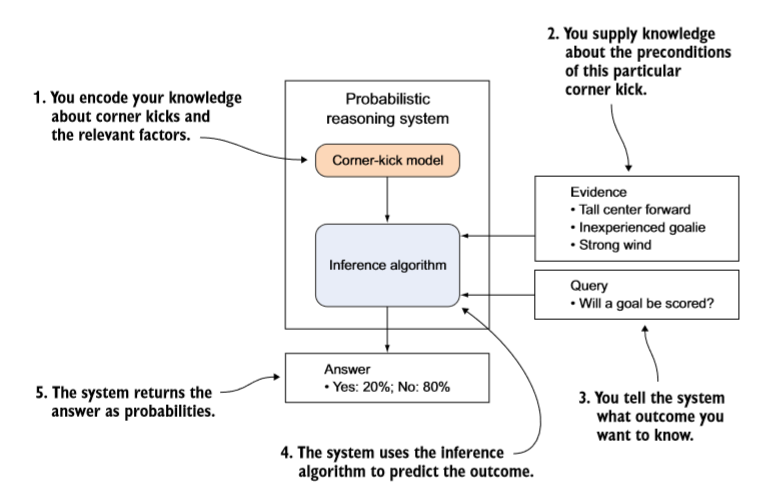
\includegraphics[width=\textwidth]{images/probabilistic_reasoning_system.PNG}
	\caption[General workflow example of a probabilistic reasoning system. Source: \cite{9781617292330}]{General workflow example of a probabilistic reasoning system}
	\label{fig:example_prs}
\end{figure}

\subsection{Difference to conventional Programming Languages}

When estimating parameters, not only the most likely value for the parameters is given, but also their uncertainty.

\subsection{Comparing Different Probabilistic Programming Languages}

\begin{itemize}
	\item stan for python: https://pystan.readthedocs.io/en/latest/
	\item pymc3: https://docs.pymc.io/notebooks/getting\_started.html\#Case-study-2:-Coal-mining-disasters
	\item edward: http://edwardlib.org/getting-started
	\item pyro: http://pyro.ai/
\end{itemize}

\subsubsection{Stan for python}

Stan is an open-source program written in C++ that is designed for Bayesian inference on user-specified models. It consists of the following components:
\begin{itemize}
	\item A modeling language that allows users to specify custom models
	\item An inference engine which uses Hamilton Monte Carlo methods for sampling to get an approximation for the posterior distribution
	\item An L-BFGS optimizer for finding local optima
	\item Procedures for automatic differentiation which are able to compute gradients required by the sampler and the optimizer
	\item Routines to monitor the convergence of parallel chains and compute inferences and effective sample sizes
	\item Wrappers for Python, R, Julia and other languages
\end{itemize}
The code for describing a model by using the aforementioned modeling language is divided into six blocks: \textit{data}, \textit{transformed data}, \textit{parameters}, \textit{transformed parameters}, \textit{model}, and \textit{generated quantities}: In \textit{data} and \textit{transformed data}, the structure of the input data, along with any constraints, is given. The difference between the former and the latter is that variables in \textit{transformed data} are functions of other data variables, whereas variables in \textit{data} are not. For example if in \textit{data}, a variable $x$ is listed, then in \textit{transformed data} one can specify a variable $y=x^2$. In \textit{parameters} and \textit{transformed parameters}, the parameters of the models are described, whereat, as in the data blocks, the latter contains variables that are functions of other parameters. In \textit{model}, the model structure in the form of prior and likelihood distributions is given. Finally, the block \textit{generated quantities} can be used to perform simulations and make predictions. In \ref{fig:stan_example_code}, an example from \cite{Gelman_2015} is shown, where the model $y=a_1e^{-b_1x} + a_2e^{-b_2x}$ is fit to data, using the PyStan interface of Stan for Python. Since not all of the aforementioned blocks are mandatory, only four of them are used in the example.
\\
PyStan also provides basic plotting methods for the posterior distributions of the parameters.

is not able to perform inference on discrete parameters. Discrete data and discrete-data models, however, are possible

computes the log-posterior density

\cite{Gelman_2015}

\cite{Hoover2016}

für den Code evtl. https://github.com/stephen-hoover/presentations zitieren

\begin{figure}
	\begin{lstlisting}
	# Specify model
	example_code = """
	data {
	// Define input data in this block
	int N;
	vector[N] x;
	vector[N] y;
	}
	parameters {
	// These are random parameters which we want to estimate
	vector[2] log_a;
	ordered[2] log_b;
	real<lower=0> sigma;
	}
	transformed parameters {
	// Create quantities derived from the parameters.
	vector<lower=0>[2] a;
	vector<lower=0>[2] b;
	a <- exp(log_a);
	b <- exp(log_b);
	}
	model {
	// Define your model here
	vector[N] ypred;
	ypred <- a[1]*exp(-b[1]*x) + a[2]*exp(-b[2]*x);
	y ~ lognormal(log(ypred), sigma);
	log_a ~ normal(0,1); 
	log_b ~ normal(0,1);
	}
	"""
	
	# Pass data to the model. x and y are the observed data
	example_dat = {'x':x,'y':y,'N':len(x)}
	# Fit model
	sm = pystan.StanModel(model_code=example_code)
	fit = sm.sampling(data=example_dat, iter=1000, chains=4)
	print(fit)
	\end{lstlisting}
	\label{fig:stan_example_code}
	\caption[Example code of a simple Bayesian model using Stan]{Example code of a simple Bayesian model using Stan}
\end{figure}

\subsubsection{Pymc3}

PyMC3 is an open-source probabilistic programming framework for Python. The following explanations are taken from \cite{Salvatier2016}. Specification of Bayesian models in PyMC3 is done by encoding the prior, the sampling and the posterior distributions through three types of random variables: Stochastic, deterministic and observed stochastic ones. Stochastic random variables have values which are in part determined randomly, according to a chosen distribution. Commonly used probability distributions like Normal, Binomial etc. are available for this. Deterministic random variables, on the other hand, are not drawn from a distribution, but are calculated by fixed rules from other variables, for example by taking the sum of two variables. Lastly, there are the observed stochastic random variables which are similar to stochastic random variables, except that they get passed observed data as an argument, that should not be changed by any fitting algorithm.  This kind of random variable can be used to represent sampling distributions.
\\
PyMC3 mainly uses simulation techniques to draw inference on posterior distributions. It focuses especially on the No-U-Turn Sampler, a Markov Chain Monte Carlo algorithm, that relies on automated differentiation to get gradient information about continuous posterior distributions. PyMC3 also provides basic methods for plotting posterior distributions.
\\
The code piece  in \ref{fig:pymc3_example_code} shows a simple example of a Bayesian model, taken from \cite{Salvatier2016}. There, the data X1, X2 and Y is used to fit a regression model. First, prior distributions for the model parameters are set up as stochastic random variables, then the regression model itself is specified by a deterministic random variable and lastly the sampling distribution is described by an observed stochastic random variable to which the observed outcome Y is given as a parameter. Finally, the posterior distribution is simulated by drawing 500 samples from it.

\begin{figure}
	\begin{lstlisting}
	import pymc3 as pm
	
	basic_model = pm.Model()
	
	with basic_model:
	# describe prior distributions of model parameters. Stochastic variables
	alpha = pm.Normal('alpha', mu=0, sd=10)
	beta = pm.Normal('beta', mu=0, sd=10, shape=2)
	sigma = pm.HalfNormal('sigma', sd=1)
	# specify model for the output parameter. Deterministic variable
	mu = alpha + beta[0]*X1 + beta[1]*X2
	# likelihood of the observations. Observed stochastic variable
	Y_obs = pm.Normal('Y_obs', mu=mu, sd=sigma, observed=Y)
	
	# model fitting by using sampling strategies   
	with basic_model:
	# draw 500 posterior samples
	trace = pm.sample(500)
	pm.summary(trace)
	\end{lstlisting}
	\label{fig:pymc3_example_code}
	\caption[Example code of a simple Bayesian model using PyMC3]{Example code of a simple Bayesian model using PyMC3}
\end{figure}

strictly positive priors are transformed with log transformation, so that they are unconstrained, since that is better for sampling

There is the possibility to create own theano functions in python. Gradient based sampling methods don't work for user-defined functions however, except when a gradient is explicitly added.

Similarily pmc3 allows to define own distributions
\subsubsection{Edward}

\subsubsection{Pyro}
\subsubsection{BUGS and Jags}
mentioned in \cite{Gelman_2015}
based on graphical models

\section{Lumen}

\textit{In this section, the Software Lumen is introduced and its abilities and uses are elucidated, especially its potential uses for Bayesian model checking in conjunction with PPLs. This covers also the theoretical aspect: Which distribution do we want to visualize with Lumen and how do we get it (using the formula $P(y,\theta|Y) = P(y|\theta) * P(\theta|Y)$)? It is outlined, what the goal of the thesis is precisely, in other words what possibilities should the interface ideally give to a user who has written a model with a PPL. Too achieve this is goal it is necessary to understand how Lumen works, so the functionality of Lumen is also explained here.} 
\\
\\
uses modelbase as backend: modelbase is a python package that provides means for fitting models to data and manipulate models by marginalization and conditionalization.


\subsection{Functionality}

In the modelbase repository, a model class is described by a python file that includes a class with several prescribed methods \url{https://ci.inf-i2.uni-jena.de/gemod/modelbase/blob/master/mb_modelbase/models_core/models.py} is a template for such a model class file, where all important methods are explained.
\\
The first step would be to implement a model there that is built by using a PPL. Then make sure that all necessary methods are correctly implemented and the visualization works as expected. One of the advantages of PPLs is the flexibility of the models specified, which is nullified by describing one fixed model. Therefore, the next steop is about thinking about a possibility to pass more flexible models. Maybe a function where you just give a model object as input that then automatically generates the necessary methods for the use in lumen??  Other possibilities? (would be good to ask that at the presentation)




compare to the plotting methods of PyMC3 / Stan

\subsection{Requirements for a PPL}

possible criterium: variety of distributions that can be described?




\section{Practical implementation}

\textit{In this section, the choices and attempts made during the practical implementation of the interface are elucidated. At first, the choice of the PPL is justified.}

\subsection{Choose the PPL for the task at hand}

\section{Case examples}

\textit{Here, case examples are presented to show how the finished interface performs in practice.}

\section {Conclusion}

\textit{In this section, the result of the thesis is summarized (and maybe also the workflow leading to it?). It is possible to understand the main ideas and results of the thesis by reading only the introduction and this section.}

\listoffigures
        
\section{Literatur}

\bibliography{Literatur.bib}
\bibliographystyle{ieeetr}


\end{document}